\documentclass[tikz]{standalone}
\usepackage{pgfplots}
\pgfplotsset{compat=1.15}
\usepackage{mathrsfs}
\usetikzlibrary{arrows,calc}
\usepackage{tkz-euclide}

\pagestyle{empty}

\definecolor{AngleClr}{rgb}{0,0.39215686274509803,0}
\definecolor{ShapeClr}{rgb}{0.6,0.2,0}
\definecolor{BlueClr}{RGB}{13,93,184}
\definecolor{RedClr}{RGB}{204, 0, 0}

\begin{document}

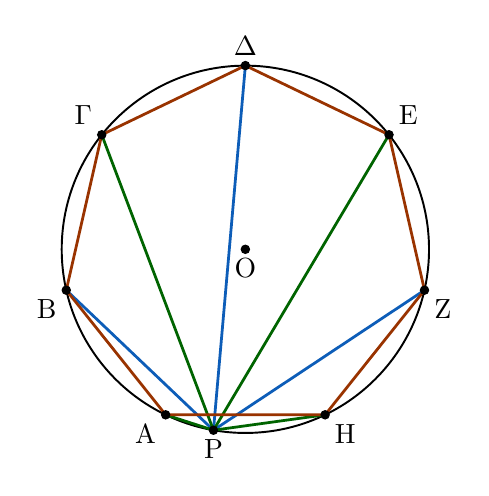
\begin{tikzpicture}[scale=.75]
\tkzSetUpLine[line width=1pt,color=black]
\tkzSetUpPoint[fill=black]

\tkzDefPoints{0/0/P0,2.7/0/P1}

\tkzDefRegPolygon[side,sides=7](P0,P1)

\tkzDefCircle[circum](P1,P2,P3) \tkzGetPoint{O}
\tkzCalcLength(O,P1)\tkzGetLength{R}

\tkzDefShiftPoint[O](-100:\R){P}

\tkzFillPolygon[fill=white](P1,P2,P3,P4,P5,P6,P7)

\tkzDrawCircle[line width=0.7pt,black](O,P1)

\tkzDrawSegments[color=BlueClr](P,P3 P,P5 P,P7)
\tkzDrawSegments[color=AngleClr](P,P1 P,P6 P,P4 P,P2)

\tkzDrawPolygon[color=ShapeClr](P1,P2,P3,P4,P5,P6,P7)
\tkzDrawPoints[size=3](P1,P2,P3,P4,P5,P6,P7,O,P)
\tkzLabelPoint[below left](P1){$\rm A$}
\tkzLabelPoint[below right](P2){$\rm H$}
\tkzLabelPoint[below right](P3){$\rm Z$}
\tkzLabelPoint[above right](P4){$\rm E$}
\tkzLabelPoint[above](P5){$\rm \Delta$}
\tkzLabelPoint[above left](P6){$\rm \Gamma$}
\tkzLabelPoint[below left](P7){$\rm B$}
\tkzLabelPoint[below](P){$\rm P$}

\tkzLabelPoint[below](O){$\rm O$}

\end{tikzpicture}

\end{document}

